\documentclass[journal,12pt,onecolumn]{IEEEtran}
\usepackage{cite}
\usepackage{amsmath,amssymb,amsfonts,amsthm}
\usepackage{algorithmic}
\usepackage{graphicx}
\usepackage{textcomp}
\usepackage{xcolor}
\usepackage{txfonts}
\usepackage{listings}
\usepackage{enumitem}
\usepackage{mathtools}
\usepackage{gensymb}
\usepackage{comment}
\usepackage[breaklinks=true]{hyperref}
\usepackage{tkz-euclide} 
\usepackage{listings}
\usepackage{gvv}                                        
                                 
\usepackage[latin1]{inputenc}     
\usepackage{xparse}
\usepackage{color}                     

\usepackage{array}                                            
\usepackage{longtable}                                        
\usepackage{calc}                
                             
\usepackage{multirow}
\usepackage{multicol}
\usepackage{hhline}                                           
\usepackage{ifthen}                            
               
\usepackage{lscape}
\usepackage{tabularx}
\usepackage{float}
\usepackage{circuitikz}
\usepackage{tikz}

\newtheorem{theorem}{Theorem}[section]
\newtheorem{problem}{Problem}
\newtheorem{proposition}{Proposition}[section]
\newtheorem{lemma}{Lemma}[section]
\newtheorem{corollary}[theorem]{Corollary}
\newtheorem{example}{Example}[section]
\newtheorem{definition}[problem]{Definition}
\newcommand{\BEQA}{\begin{eqnarray}}
\newcommand{\EEQA}{\end{eqnarray}}
%\newcommand{\define}{\stackrel{\triangle}{=}}
\theoremstyle{remark}
%\newtheorem{rem}{Remark}

\begin{document}
\title{GATE $2025$ Geomatics Engineering (GE)}
\author{EE$25$BTECH$11033$- Kavin B}
\maketitle
\renewcommand{\thefigure}{\theenumi}
\renewcommand{\thetable}{\theenumi}

\underline{\textbf{General Aptitude (GA)}}
\\

\textbf{Q.$1$ $-$ Q.$5$ Carry ONE mark Each}
\vspace{0.5cm}
\begin{enumerate}
\item Here are two analogous groups, Group-I and Group-II, that list words in their decreasing order of intensity. Identify the missing word in Group-II.\\
\\
\noindent Group-I: \quad Abuse $\rightarrow$ Insult $\rightarrow$ Ridicule \\
Group-II: \quad \rule{1.5cm}{0.15mm} $\rightarrow$ Praise $\rightarrow$ Appreciate

\begin{enumerate}
\begin{multicols}{4}
\item Extol
\item Prize
\item Appropriate
\item Espouse
\end{multicols}
\end{enumerate}
\hfill $\brak{\text{GATE GE 2025}}$
\bigskip
\item Had I learnt acting as a child, I \rule{2.5cm}{1pt} a famous film star.
\begin{enumerate}
\begin{multicols}{4}
\item will be
\item can be
\item am going to be
\item could have been
\end{multicols}
\end{enumerate}
\hfill $\brak{\text{GATE GE 2025}}$
\bigskip
\item The 12 musical notes are given as $C, C^\#, D, D^\#, E, F, F^\#, G, G^\#, A, A^\#$, and $B$. Frequency of each note is $\frac{12\sqrt{2}}{2}$ times the frequency of the previous note. If the frequency of the note $C$ is 130.8 Hz, then the ratio of frequencies of notes $F^\#$ and $C$ is:
\begin{enumerate}
\begin{multicols}{4}
\item $\sqrt[6]{2}$
\item $\sqrt{2}$
\item $\sqrt[4]{2}$
\item $2$
\end{multicols}
\end{enumerate}
\hfill $\brak{\text{GATE GE 2025}}$
\bigskip

\item The following figures show three curves generated using an iterative algorithm. The total length of the curve generated after 'Iteration $n$' is:\\
\\
Note: The figures shown are representative.\\
\begin{figure}[H]
    \centering
    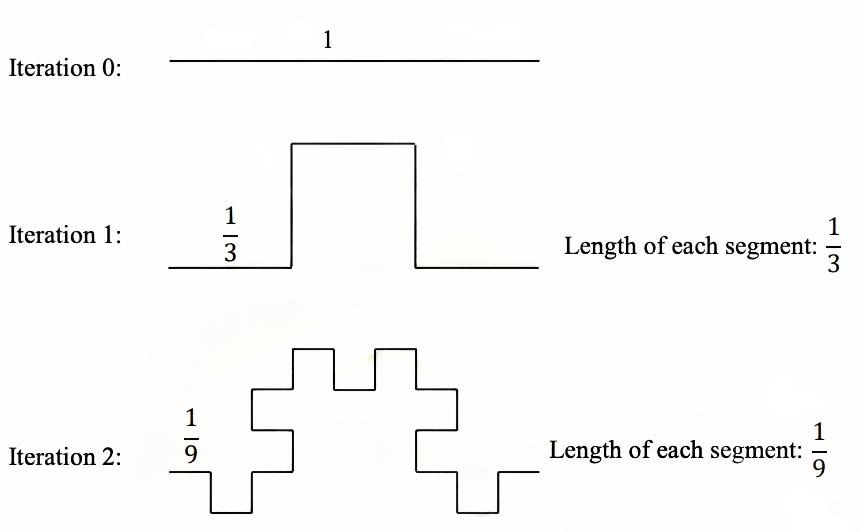
\includegraphics[width=0.6\columnwidth]{figs/fig1.png}
    \caption{Figure}
    \label{figs:fig1}
\end{figure}

\begin{enumerate}
\begin{multicols}{4}
\item $\sqrt[5]{\frac{n}{2}}$
\item $\sqrt[5]{\frac{n}{3}}$
\item $\sqrt[5]{\frac{2n}{3}}$
\item $\sqrt[5]{\frac{n(2n-1)}{3}}$
\end{multicols}
\end{enumerate}
\hfill $\brak{\text{GATE GE 2025}}$
\bigskip
\item Which one of the following plots represents $f(x) = -\frac{|x|}{x}$, where $x$ is a non-zero real number?
\begin{enumerate}
\begin{multicols}{4}
\item 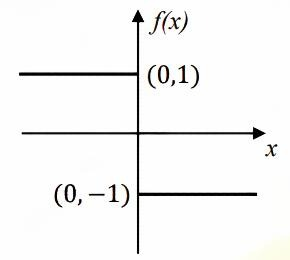
\includegraphics[width=0.7\columnwidth]{figs/figA.png}
\item 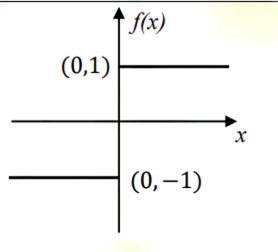
\includegraphics[width=0.7\columnwidth]{figs/figB.png}
\item 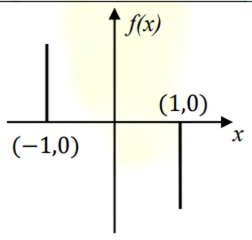
\includegraphics[width=0.7\columnwidth]{figs/figC.png}
\item 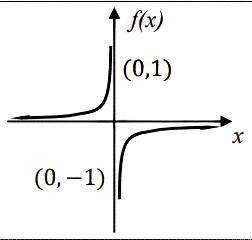
\includegraphics[width=0.7\columnwidth]{figs/figD.png}
\end{multicols}
\end{enumerate}
\hfill $\brak{\text{GATE GE 2025}}$
\bigskip
\end{enumerate}

\textbf{Q.$6$ $-$ Q.$10$ Carry TWO marks Each}\\
\begin{enumerate}
\setcounter{enumi}{5}
\item Identify the option that has the most appropriate sequence such that a coherent paragraph is formed:\\
P. Over time, such adaptations lead to significant evolutionary changes with the potential to shape the development of new species.\\
Q. In natural world, organisms constantly adapt to their environments in response to challenges and opportunities.\\
R. This process of adaptation is driven by the principle of natural selection, where favorable traits increase an organism's chances of survival and reproduction.\\
S. As environments change, organisms that can adapt their behavior, structure and physiology to such changes are more likely to survive.
\begin{enumerate}
\item P $\rightarrow$ Q $\rightarrow$ R $\rightarrow$ S
\item Q $\rightarrow$ S $\rightarrow$ R $\rightarrow$ P
\item R $\rightarrow$ S $\rightarrow$ Q $\rightarrow$ P
\item S $\rightarrow$ P $\rightarrow$ R $\rightarrow$ Q
\end{enumerate}
\hfill $\brak{\text{GATE GE 2025}}$
\bigskip
\item A stick of length one meter is broken at two locations at distances of $b_1$ and $b_2$ from the origin (0), as shown in the figure. Note that $0 < b_1 < b_2 < 1$. Which one of the following is NOT a necessary condition for forming a triangle using the three pieces?\\
\\
Note: All lengths are in meter. The figure shown is representative.\\
\begin{figure}[H]
    \centering
    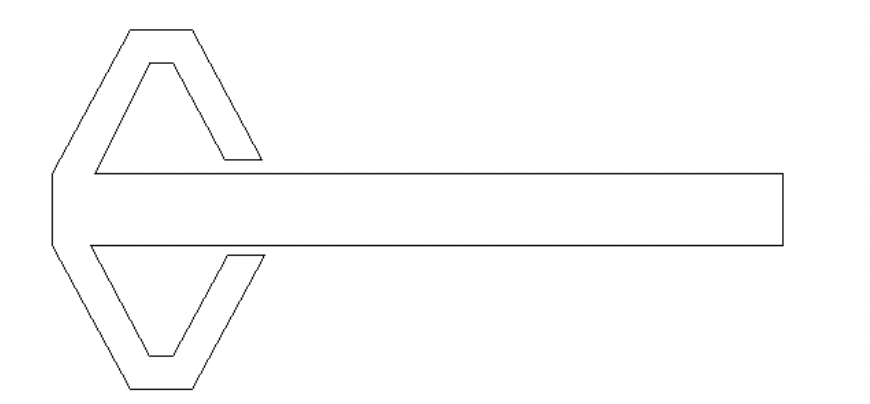
\includegraphics[width=0.7\columnwidth]{figs/fig2.png}
    \caption{\centering{Figure}}
    \label{figs:fig12}
\end{figure}
\begin{enumerate}
\begin{multicols}{4}
\item $b_1 < 0.5$
\item $b_2 > 0.5$
\item $b_2 < b_1 + 0.5$
\item $b_1 + b_2 < 1$
\end{multicols}
\end{enumerate}
\hfill $\brak{\text{GATE GE 2025}}$
\bigskip
\item Eight students (P, Q, R, S, T, U, V, and W) are playing musical chairs. The figure indicates their order of position at the start of the game. They play the game by moving forward in a circle in the clockwise direction.\\
\\
After the $1^{\text{st}}$ round, $4^{\text{th}}$ student behind P leaves the game. After $2^{\text{nd}}$ round, $5^{\text{th}}$ student behind Q leaves the game. After $3^{\text{rd}}$ round, $3^{\text{rd}}$ student behind V leaves the game. After $4^{\text{th}}$ round, $4^{\text{th}}$ student behind U leaves the game. Who all are left in the game after the $4^{\text{th}}$ round?\\
\\
Note: The figure shown is representative.\\
\begin{figure}[H]
    \centering
    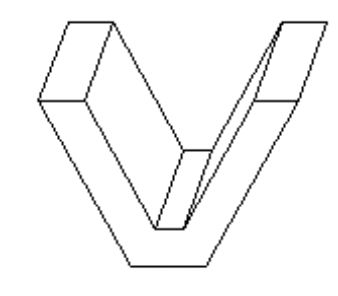
\includegraphics[width=0.4\columnwidth]{figs/fig3.png}
    \caption{\centering{Figure}}
    \label{figs:fig3}
\end{figure}
\begin{enumerate}
\begin{multicols}{4}
\item P; T; Q; S
\item V; P; T; Q
\item W; R; Q; V
\item Q; T; V; W
\end{multicols}
\end{enumerate}
\hfill $\brak{\text{GATE GE 2025}}$
\bigskip
\item The table lists the top 5 nations according to the number of gold medals won in a tournament; also included are the number of silver and the bronze medals won by them. Based only on the data provided in the table, which one of the following statements is INCORRECT?
\begin{table}[h]
\centering
\begin{tabular}{|c|c|c|c|}
\hline
Nation & Gold & Silver & Bronze \\
\hline
USA & 40 & 44 & 41 \\
Canada & 39 & 27 & 24 \\
Japan & 20 & 12 & 13 \\
Australia & 17 & 19 & 16 \\
France & 16 & 26 & 22 \\
\hline
\end{tabular}
\end{table}
\begin{enumerate}
\item France will occupy the third place if the list were made on the basis of the total number of medals won.
\item The order of the top two nations will not change even if the list is made on the basis of the total number of medals won.
\item USA and Canada together have less than 50\% of the medals awarded to the nations in the above table.
\item Canada has won twice as many total medals as Japan.
\end{enumerate}
\hfill $\brak{\text{GATE GE 2025}}$
\bigskip
\item An organization allows its employees to work independently on consultancy projects but charges an overhead on the consulting fee. The overhead is 20\% of the consulting fee, if the fee is up to 
\rupee500000. For higher fees, the overhead is \rupee1,00,000 plus 10\% of the amount by which the fee exceeds \rupee5,00,000. The government charges a Goods and Services Tax of 18\% on the total amount (the consulting fee plus the overhead). An employee of the organization charges this entire amount, i.e., the consulting fee, overhead, and tax, to the client. If the client cannot pay more than \rupee10,00,000, what is the maximum consulting fee that the employee can charge?
\begin{enumerate}
\begin{multicols}{4}
\item \rupee7,01,438
\item \rupee7,24,961
\item \rupee7,51,232
\item \rupee7,75,784
\end{multicols}
\end{enumerate}
\hfill $\brak{\text{GATE GE 2025}}$
\bigskip
\end{enumerate}

\textbf{PART A: Common FOR ALL CANDIDATES}\\
\\
\textbf{Q.$11$ $-$ Q.$27$ Carry ONE mark Each}\\

\begin{enumerate}
\setcounter{enumi}{10}
\item For a sample drawn from normally distributed population, the statistic $Y = \frac{(n-1)s^2}{\sigma^2}$, where $n =$ sample size, $\sigma =$ population standard deviation, $s =$ sample standard deviation, has
\begin{enumerate}
\item Chi-square distribution with $(n-1)$ degrees of freedom
\item Chi-square distribution with $n$ degrees of freedom
\item Chi-square distribution with $(n+1)$ degrees of freedom
\item Gaussian distribution with $n$ degrees of freedom
\end{enumerate}
\hfill $\brak{\text{GATE GE 2025}}$
\bigskip
\item The reflectance geometry of white-sky albedo can be represented as \rule{2cm}{0.5mm}.
\begin{enumerate}
\begin{multicols}{4}
\item bi-directional
\item bi-conical
\item bi-hemispherical
\item directional-conical
\end{multicols}
\end{enumerate}
\hfill $\brak{\text{GATE GE 2025}}$
\bigskip
\item Clouds appear white in optical visible spectral bands of remote sensing images due to \rule{2cm}{0.5mm} scattering.
\begin{enumerate}
\begin{multicols}{4}
\item Rayleigh
\item Mie
\item selective
\item non-selective
\end{multicols}
\end{enumerate}
\hfill $\brak{\text{GATE GE 2025}}$
\bigskip
\item If the absolute temperature (greater than 0 K) of a body is doubled, it would emit \rule{2cm}{0.5mm} times more radiation.
\begin{enumerate}
\begin{multicols}{4}
\item 2
\item 4
\item 8
\item 16
\end{multicols}
\end{enumerate}
\hfill $\brak{\text{GATE GE 2025}}$
\bigskip
\item If the emissivity of an object varies with wavelength, it is called as \rule{2cm}{0.5mm}.
\begin{enumerate}
\begin{multicols}{4}
\item grey body
\item black body
\item selective radiant
\item non-selective radiant
\end{multicols}
\end{enumerate}
\hfill $\brak{\text{GATE GE 2025}}$
\bigskip
\item In the context of Global Navigation Satellite System positioning, the Saastamoinen model provides a correction for \rule{2cm}{0.5mm}.
\begin{enumerate}
\begin{multicols}{4}
\item zenith hydrostatic delay
\item slant hydrostatic delay
\item zenith total delay
\item slant total delay
\end{multicols}
\end{enumerate}
\hfill $\brak{\text{GATE GE 2025}}$
\bigskip
\item In the context of Global Navigation Satellite System positioning, which of the following statement is correct?
\begin{enumerate}
\item In Differential Global Navigation Satellite System, the corrections to the coordinates of the user are transmitted from the reference station
\item Real-time kinematic positioning and stop-and-go positioning are both kinematic methods
\item Rapid-static positioning is not a relative positioning technique
\item Double differencing eliminates the clock errors and improves the noise in the differenced pseudorange observations
\end{enumerate}
\hfill $\brak{\text{GATE GE 2025}}$
\bigskip
\item In the choke ring antenna there are concentric cylinders placed around the antenna that are of a certain depth to minimize the multipath effect. If the signal wavelength is $\lambda$, then the depth of the cylinders in the choke ring antenna should be
\begin{enumerate}
\begin{multicols}{4}
\item exactly $\frac{\lambda}{4}$
\item slightly more than $\frac{\lambda}{4}$ and far less than $\frac{\lambda}{2}$
\item exactly $\frac{\lambda}{2}$
\item slightly more than $\frac{\lambda}{2}$ and far less than $\lambda$
\end{multicols}
\end{enumerate}
\hfill $\brak{\text{GATE GE 2025}}$
\bigskip
\item Which one of the following statements is NOT correct in the context of Geographic Information System?
\begin{enumerate}
\item A raster data model makes use of grid of cells that are organized into rows and columns for representation of features on earth
\item Vector data model represents the spatial features on Earth's surface in terms of points, lines or polygons
\item Resampling is applied after georeferencing of vector datasets
\item Topology is used in vector data models to ensure spatial data integrity
\end{enumerate}
\hfill $\brak{\text{GATE GE 2025}}$
\bigskip
\item Which one of the following statements is NOT correct in the context of shapefile?
\begin{enumerate}
\item It is an example of georelational data model
\item It is a topological data model
\item It treats points as pairs of (x, y) coordinates
\item In this, polygons can have duplicate arcs for shared boundaries
\end{enumerate}
\hfill $\brak{\text{GATE GE 2025}}$
\bigskip
\item The table below is an attribute table about employee records. Which attribute can be used as a primary key?
\begin{table}[h]
\centering
\begin{tabular}{|c|c|c|c|}
\hline
Emp\_ID & Emp\_Name & Emp\_Design & Emp\_Dept \\
\hline
100260 & Prashant & Software Developer & Information Technology \\
100265 & Dinesh & Junior Engineer & Embedded System \\
100252 & Somya & HR Manager & Management \\
100271 & Dinesh & Junior Engineer & Information Technology \\
\hline
\end{tabular}
\end{table}
\begin{enumerate}
\begin{multicols}{4}
\item Emp\_Name
\item Emp\_ID
\item Emp\_Dept
\item Emp\_Design
\end{multicols}
\end{enumerate}
\hfill $\brak{\text{GATE GE 2025}}$
\bigskip
\item Find the best match between column I and column II for the following scenario related to spatial operators.
\begin{figure}[H]
    \centering
    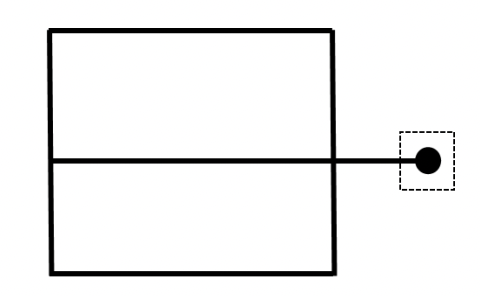
\includegraphics[width=0.2\columnwidth]{figs/fig4.png}
    \caption{\centering{Figure}}
    \label{figs:fig4}
\end{figure}
\begin{figure}[H]
    \centering
    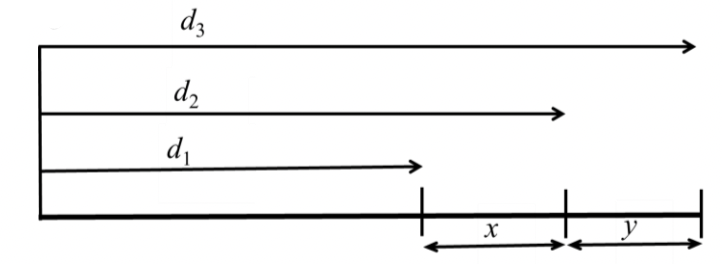
\includegraphics[width=0.4\columnwidth]{figs/fig5.png}
    \caption{\centering{Figure}}
    \label{figs:fig5}
\end{figure}
\begin{enumerate}
\begin{multicols}{4}
\item P-2; Q-3; R-1
\item P-1; Q-3; R-2
\item P-2; Q-1; R-3
\item P-1; Q-2; R-3
\end{multicols}
\end{enumerate}
\hfill $\brak{\text{GATE GE 2025}}$
\bigskip
\item For the weighted least squares adjustment, which of the following statements is/are correct?
\begin{enumerate}
\item Weighted sum of the squares of the residuals is minimized
\item The expected value of the residuals is equal to zero
\item Redundancy of observations is maximized
\item Weights are taken inversely proportional to the variance of the observations
\end{enumerate}
\hfill $\brak{\text{GATE GE 2025}}$
\bigskip
\item The geophysical variables that can be measured/derived from the Global Navigation Satellite System observations is/are
\begin{enumerate}
\item ocean color
\item precipitable water vapor
\item soil moisture
\item seismic motion
\end{enumerate}
\hfill $\brak{\text{GATE GE 2025}}$
\bigskip
\item For a given set of observations for distance measurements, the standard error was computed as $\pm 2.5$ cm. Assuming that the observations conform to normal error distribution theory, the probable error will be given by $\pm$ \rule{2cm}{0.5mm} cm (rounded off to 2 decimal places).
\\
\\.
\hfill $\brak{\text{GATE GE 2025}}$
\bigskip
\item In a two-dimensional coordinate system, it is proposed to determine the size and shape of a triangle ABC in addition to its location and orientation. For this, all the internal angles and sides of the triangle were observed. Further, the planar coordinates of point A and bearing/azimuth of line AB were known. The redundancy (r) for the above system will be equal to \rule{2cm}{0.5mm} (Answer in integer).
\\
\\.
\hfill $\brak{\text{GATE GE 2025}}$
\bigskip
\item The covariance matrix, $\Sigma$, for the planar coordinates of a surveyed point is given as:
\[
\Sigma = 
\myvec{
25  \text{mm}^2 & 0.500  \text{mm}^2 \\
0.500  \text{mm}^2 & 100  \text{mm}^2
}
\]
The coefficient of correlation is \rule{2cm}{0.5mm} (rounded off to 2 decimal places).
\\
\\.
\hfill $\brak{\text{GATE GE 2025}}$
\bigskip
\end{enumerate}

\textbf{Q.$28$ $-$ Q.$46$ Carry TWO marks Each}\\
\begin{enumerate}
\setcounter{enumi}{27}
\item Match the following SAR sensors to their frequency bands
\begin{table}[h]
\centering
\begin{tabular}{|c|c|}
\hline
Column I & Column II \\
\hline
P NOVASAR & 1 X-BAND \\
Q RISAT-1 & 2 C-BAND \\
R TERRASAR & 3 L-BAND \\
S ALOS PALSAR & 4 S-BAND \\
\hline
\end{tabular}
\end{table}
\begin{enumerate}
\begin{multicols}{4}
\item P-3, Q-2, R-4, S-1
\item P-4, Q-2, R-1, S-3
\item P-2, Q-4, R-1, S-3
\item P-1, Q-4, R-3, S-2
\end{multicols}
\end{enumerate}
\hfill $\brak{\text{GATE GE 2025}}$
\bigskip
\item The relativistic effect in Global Navigation Satellite System satellites has two parts, of which the first part is the time dilation due to the shift in the fundamental frequency of the satellite clock. The second part is due to the satellite's semi-major axis and \rule{2cm}{0.5mm}.
\begin{enumerate}
\begin{multicols}{2}
\item eccentricity
\item inclination
\item argument of perigee
\item right ascension of the ascending node
\end{multicols}
\end{enumerate}
\hfill $\brak{\text{GATE GE 2025}}$
\bigskip
\item A country has 7 permanent Global Navigation Satellite System stations covering its territory. Their surveying organization generates a network solution after applying double differencing to the observations. These 7 permanent stations can view 5 to 10 common satellites at any given epoch. What is the range (minimum, maximum) of the number of independent double differenced observables possible?
\begin{enumerate}
\begin{multicols}{4}
\item \brak{35,70}
\item \brak{30,56}
\item \brak{28,48}
\item \brak{24,54}
\end{multicols}
\end{enumerate}
\hfill $\brak{\text{GATE GE 2025}}$
\bigskip
\item Consider the nodes of a square grid A, B, C and D (shown in figure below), where a certain parameter is measured. The distances between the points is also indicated in the same figure. For example, the value observed at point A is 120 and is indicated as A (120), and the distance between points A and B is 1.0 units. The value at point 'X' computed using bilinear interpolation, using the values at points A, B, C and D is \rule{2cm}{0.5mm}.
\begin{figure}[H]
    \centering
    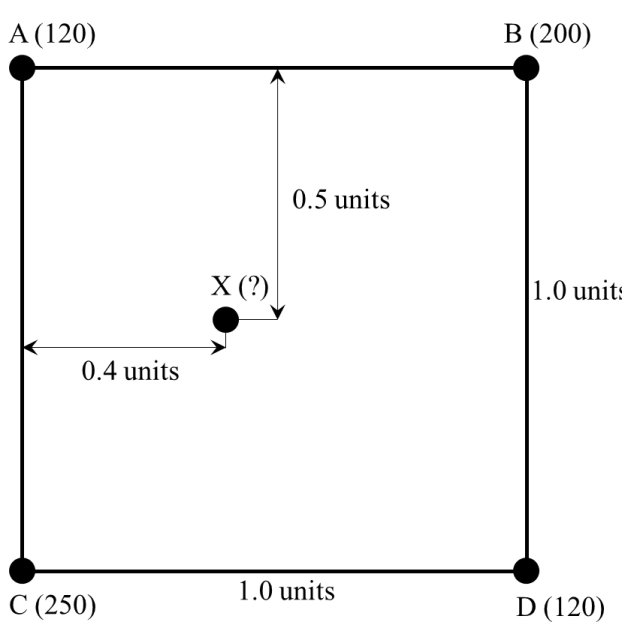
\includegraphics[width=0.4\columnwidth]{figs/fig6.png}
    \caption{\centering{Figure}}
    \label{figs:fig6}
\end{figure}
\begin{enumerate}
\begin{multicols}{4}
\item 175
\item 152
\item 198
\item 210
\end{multicols}
\end{enumerate}
\hfill $\brak{\text{GATE GE 2025}}$
\bigskip
\item The first value in the output of a SQL query (given below) when run on a table having name "Table-1" is?
\begin{verbatim}
SQL Query: SELECT LastName FROM Table-1 WHERE State="IN" ORDER BY FirstName
\end{verbatim}
\begin{table}[h]
\centering
\begin{tabular}{|c|c|c|c|c|c|}
\hline
LastName & FirstName & StreetNumber & StreetName & City & State \\
\hline
Squires & Edwin & 4589 & Shamar Rd. & Upland & IN \\
Rothrock & Paul & 91657 & Carex Ave. & Upland & IN \\
Ramirez & Douglas & 123 & Fake St. & Springfield & IN \\
Peterson & Chris & 4687 & Windthrow Way & Kane & PA \\
Gibson & David & 354 & Bluestem St. & Carbondale & IL \\
\hline
\end{tabular}
\end{table}
\begin{enumerate}
\begin{multicols}{4}
\item Ramirez
\item Douglas
\item Paul
\item Squires
\end{multicols}
\end{enumerate}
\hfill $\brak{\text{GATE GE 2025}}$
\bigskip
\item Consider the three input raster images given below. A geospatial analyst decided to use the overlay operation to generate a new raster showing the average values. The values of the cells P, Q and R in the output raster are:
\begin{figure}[H]
    \centering
    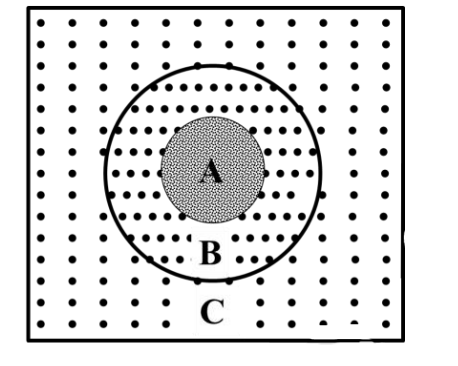
\includegraphics[width=0.4\columnwidth]{figs/fig10.png}
    \caption{\centering{Figure}}
    \label{figs:fig10}
\end{figure}

\begin{enumerate}
\begin{multicols}{4}
\item P = 3, Q = 3, R = 2
\item P = 4, Q = 4, R = 3
\item P = 3, Q = 3, R = 3
\item P = 4, Q = 4, R = 2
\end{multicols}
\end{enumerate}
\hfill $\brak{\text{GATE GE 2025}}$
\bigskip
\item In a Geographic Information System database, a stream is represented by a line and houses are represented by polygons. The pollution in the stream is affecting houses within a distance of 500 m on both sides. Which vector data analysis operations should be performed to identify houses affected by the pollution in the stream?
\begin{enumerate}
\begin{multicols}{4}
\item Buffer and Overlay
\item Dissolve and Overlay
\item Buffer
\item Split
\end{multicols}
\end{enumerate}
\hfill $\brak{\text{GATE GE 2025}}$
\bigskip
\item In a given weighted graph shown below, what is the value of the expression $(p + d)^2$ where,\\
i. Alphabets A, B, C, D, E and F denote the nodes\\
ii. Numbers 1 to 6 denote the weights between two nodes\\
iii. $d =$ shortest distance between node A and node E\\
iv. $p =$ number of paths with distance $d$
\begin{figure}[H]
    \centering
    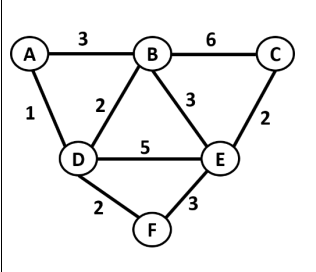
\includegraphics[width=0.4\columnwidth]{figs/fig7.png}
    \caption{\centering{Figure}}
    \label{figs:fig7}
\end{figure}
\begin{enumerate}
\begin{multicols}{4}
\item 100
\item 64
\item 81
\item 121
\end{multicols}
\end{enumerate}
\hfill $\brak{\text{GATE GE 2025}}$
\bigskip
\item In a plane triangle, the observed angles P, Q and R, assumed uncorrelated, with given weights are:\\
P = $40^\degree19'02''$ weight = 1\\
Q = $70^\degree30'01''$ weight = 2\\
R = $69^\degree11'00''$ weight = 1\\
The most probable values of these angles $(\hat{P}, \hat{Q}, \hat{R})$ will be given by:
\begin{enumerate}
\item $\hat{P} = 40^\degree19'00''$, $\hat{Q} = 70^\degree30'00''$, $\hat{R} = 69^\degree11'00''$
\item $\hat{P} = 40^\degree19'01''$, $\hat{Q} = 70^\degree30'00''$, $\hat{R} = 69^\degree10'59''$
\item $\hat{P} = 40^\degree19'0.8''$, $\hat{Q} = 70^\degree30'0.4''$, $\hat{R} = 69^\degree10'58.8''$
\item $\hat{P} = 40^\degree18'58.4''$, $\hat{Q} = 70^\degree30'0.4''$, $\hat{R} = 69^\degree11'1.2''$
\end{enumerate}
\hfill $\brak{\text{GATE GE 2025}}$
\bigskip
\item Which of the following statements is/are correct in the context of Voronoi polygon?
\begin{enumerate}
\item A Voronoi polygon may contain more than one point, especially where the density of points is higher
\item The center of a Voronoi polygon is a circumcenter of a Delaunay triangle
\item Each intersection of Voronoi edges belongs to at least three Voronoi polygons
\item Voronoi polygons and Delaunay triangles are geometric dual of each other
\end{enumerate}
\hfill $\brak{\text{GATE GE 2025}}$
\bigskip
\item Which of the following conditions is/are essential for geostationary satellite orbits?
\begin{enumerate}
\item Eccentricity is zero
\item Inclination is close to zero
\item Prograde
\item Retrograde
\end{enumerate}
\hfill $\brak{\text{GATE GE 2025}}$
\bigskip
\item Two adjacent angles $A$ and $B$ have been observed with the following mean values and correlation matrix, $\rho$:
\[
\bar{A} = 10^\degree20'10'' \pm 10''
\]
\[
\bar{B} = 25^\degree35'15'' \pm 20''
\]
\[
\rho = \myvec{
1.0 & 0.6 \\
0.6 & 1.0}
\]
The standard deviation of the sum of the estimated angles $\bar{A}$ and $\bar{B}$ will be \rule{2cm}{0.5mm} (in arcseconds) (rounded off to 2 decimal places).
\\
\\.
\hfill $\brak{\text{GATE GE 2025}}$
\bigskip
\item The residual error in a measurement comprises a bias of + 0.08 m and a random component given by the following density function:
\[
f(x) = \frac{1}{0.15} \exp \left( \frac{-x^2}{0.0072} \right)  \text{m}^{-1}
\]
For this system, the mean square error (MSE) is \rule{2cm}{0.5mm} m. (rounded off to 2 decimal places)
\\
\\.
\hfill $\brak{\text{GATE GE 2025}}$
\bigskip
\item For the following ten angle observations, the standard error of the mean angle is given as \rule{2cm}{0.5mm} arcsecond (rounded off to 2 decimal places).
\[
25^\degree40'12'',\   25^\degree40'14'',\  25^\degree40'16'',\   25^\degree40'18'',\   25^\degree40'09'',\ 
\]
\[
25^\degree40'15'',\   25^\degree40'10'',\   25^\degree40'13'',\   25^\degree40'15'',\   25^\degree40'18''\ 
\]
\\
\\.
\hfill $\brak{\text{GATE GE 2025}}$
\bigskip
\item The velocity ($V_s$) of a satellite moving in a circular orbit at a height of 1000 km above earth surface is \rule{2cm}{0.5mm} km s$^{-1}$ (rounded off to 2 decimal places).
\\
$(G = 6.67 \times 10^{-11}  \text{m}^3  \text{kg}^{-1}  \text{s}^{-2},  M_e = 5.972 \times 10^{24}  \text{kg}  \text{and}  r_e = 6378  \text{km})$
\\
\\.
\hfill $\brak{\text{GATE GE 2025}}$
\bigskip
\item If the radiant temperature of a body is 360 K and its emissivity 0.6, then the kinetic temperature of that body is \rule{2cm}{0.5mm} K (Answer in integer).
\\
\\.
\hfill $\brak{\text{GATE GE 2025}}$
\bigskip
\item Energy carried by a part of short-wave infrared ray at 1000 nm wavelength is \rule{2cm}{0.5mm} eV (rounded off to 2 decimal places).
\\
$(h = 6.626 \times 10^{-34}  \text{J}  \text{s},  1  \text{J} = 6.242 \times 10^{18}  \text{eV},  c = 3 \times 10^8  \text{m}  \text{s}^{-1})$
\\
\\.
\hfill $\brak{\text{GATE GE 2025}}$
\bigskip
\item The scattering matrix for a fully polarimetric synthetic aperture radar pixel is given below. The $C_{11}$ element of the covariance matrix computed with a $1 \times 1$ window will be \rule{2cm}{0.5mm}? (rounded off to 2 decimal places).
\[
\myvec{
0.1 + 0.5i & 0.1 - 0.1i \\
0.1 + 0.1i & 0.3 - 0.5i
}
\]
Here, $i = \sqrt{-1}$.
\\
\\.
\hfill $\brak{\text{GATE GE 2025}}$
\bigskip
\item Global Navigation Satellite System can be used for positioning and timing. The average geometric dilution of precision (GDOP) at a location is 1.0 and positional dilution of precision (PDOP) is 0.8. With the precision of the measurements being 300 m, the achieved precision of timing is \rule{2cm}{0.5mm} ns (Answer in integer).
\\
Consider the speed of light is $3 \times 10^8  \text{m s}^{-1}$
\\
\\.
\hfill $\brak{\text{GATE GE 2025}}$
\bigskip
\end{enumerate}

\textbf{PART B1: FOR  I: SectionSurveying and Mapping CANDIDATES ONLY}\\

\textbf{Q.$47$ $-$ Q.$54$ Carry ONE mark Each}\\
\begin{enumerate}
\setcounter{enumi}{46}
\item Two positions on the Earth's surface are given in the form of Cartesian coordinates in the WGS84 reference frame and ellipsoid. The norm of difference of these two position vectors is the\rule{2cm}{0.5mm}.
\begin{enumerate}
\begin{multicols}{4}
\item spherical distance
\item ellipsoidal distance
\item Euclidean distance
\item planar distance
\end{multicols}
\end{enumerate}
\hfill $\brak{\text{GATE GE 2025}}$
\bigskip
\item Which one of the following map projections is NOT conformal?
\begin{enumerate}
\begin{multicols}{2}
\item Transverse Mercator
\item Stereographic
\item Lambert Conformal Conic
\item Sinusoidal
\end{multicols}
\end{enumerate}
\hfill $\brak{\text{GATE GE 2025}}$
\bigskip
\item In a Survey of India topographic map of scale 1:50,000, the contours are drawn conventionally at intervals of \rule{2cm}{0.5mm} m.
\begin{enumerate}
\begin{multicols}{4}
\item 10 and 20
\item 20 and 40
\item 30 and 50
\item 25 and 50
\end{multicols}
\end{enumerate}
\hfill $\brak{\text{GATE GE 2025}}$
\bigskip
\item Figure below shows an open traverse PQRS, where P is the starting point of traverse and S is the end point of traverse. Which one of the following is correct?
\begin{figure}[H]
    \centering
    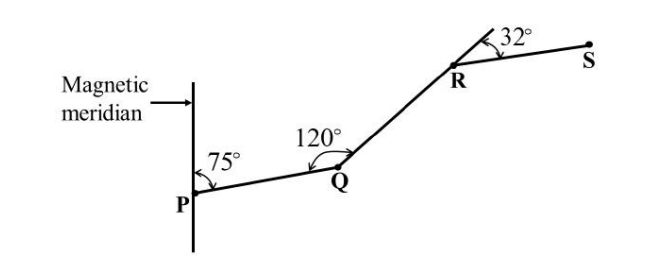
\includegraphics[width=0.4\columnwidth]{figs/fig8.png}
    \caption{\centering{Figure}}
    \label{figs:fig8}
\end{figure}
\begin{enumerate}
\item $\angle R =$ Bearing = $32^\degree$, $\angle P =$ Deflection Angle = $75^\degree$, $\angle Q =$ Included Angle = $120^\degree$
\item $\angle P =$ Bearing = $75^\degree$, $\angle Q =$ Deflection Angle = $120^\degree$, $\angle R =$ Included Angle = $32^\degree$
\item $\angle P =$ Bearing = $75^\degree$, $\angle R =$ Deflection Angle = $32^\degree$, $\angle Q =$ Included Angle = $120^\degree$
\item $\angle R =$ Bearing = $32^\degree$, $\angle Q =$ Deflection Angle = $120^\degree$, $\angle P =$ Included Angle = $75^\degree$
\end{enumerate}
\hfill $\brak{\text{GATE GE 2025}}$
\bigskip
\item When conducting a survey using a total station, a zenith angle is measured as $84^\degree13'56''$ in the direct mode. What is the equivalent zenith angle in the reverse mode?
\begin{enumerate}
\begin{multicols}{4}
\item $264^\degree13'56''$
\item $05^\degree46'04''$
\item $275^\degree46'04''$
\item $185^\degree46'04''$
\end{multicols}
\end{enumerate}
\hfill $\brak{\text{GATE GE 2025}}$
\bigskip
\item In a closed traverse PQRST the following data were collected in the field. What is the correct sum of deflection angles for this traverse?
\begin{table}[h]
\centering
\begin{tabular}{|c|c|c|}
\hline
Line & Length (m) & Bearing \\
\hline
PQ & 201.54 & $62^\degree42'$ \\
QR & 189.68 & $154^\degree54'$ \\
RS & 231.94 & $202^\degree32'$ \\
ST & 272.55 & $281^\degree44'$ \\
TP & 256.83 & $350^\degree48'$ \\
\hline
\end{tabular}
\end{table}
\begin{enumerate}
\begin{multicols}{4}
\item $382^\degree$00
\item $360^\degree$00'
\item $540^\degree$00'
\item $723^\degree$52'
\end{multicols}
\end{enumerate}
\hfill $\brak{\text{GATE GE 2025}}$
\bigskip
\item Which one of the following parameters does NOT affect the scale of a vertical aerial photograph?

\begin{enumerate}

\item Size of the photograph
\item Focal length of the camera
\item Flying height
\item Terrain elevation

\end{enumerate}
\hfill $\brak{\text{GATE GE 2025}}$
\bigskip
\item Select the correct statement in the context of relief displacement in vertical aerial photographs.
\begin{enumerate}
\item It is zero for principal point, irrespective of whether the point is above or below the datum
\item It increases with increased flying height above datum
\item It occurs radially from one of the image corners
\item It has no effect on the appearance (in the aerial photograph) of the straight roads over an undulating terrain
\end{enumerate}
\hfill $\brak{\text{GATE GE 2025}}$
\bigskip
\end{enumerate}

\textbf{Q.$55$ $-$ Q.$60$ Carry TWO marks Each}\\

\begin{enumerate}
\setcounter{enumi}{54}
\item Given $h_P = H_P + N_P$, where $h_P$ is the ellipsoidal/geodetic height at point P, $H_P$ is the orthometric height and $N_P$ is the geoid undulation along the ellipsoidal normal. Which one of the following statements is correct?
\begin{enumerate}
\item Two points on the Earth's surface that have the same ellipsoidal height will be on the same equipotential surface
\item The geoid undulation is the separation of the equipotential surface at the ground surface with respect to the ellipsoid
\item The points on an equipotential surface will not have the same orthometric height
\item The orthometric height of the instantaneous sea level is zero
\end{enumerate}
\hfill $\brak{\text{GATE GE 2025}}$
\bigskip
\item In the figure below, I1 and I2 are the two instrument stations. The instrument stations and the object (P) lie in the same vertical plane. Assume all instruments and staff are levelled. \\
\\
$L$ = horizontal distance between the object and the station I2 \\
$b$ = horizontal distance between the instrument stations \\
$S$ = staff reading at the Benchmark (BM) for horizontal line of sight \\
$H$ = reading on the staff at P \\
$r$ = height of the point sighted by instruments at the staff kept at P from the line of sight of the instruments \\
$\alpha_1$ and $\alpha_2$ = vertical angles to the reading on staff at P from I1 and I2, respectively \\
\\
Which one of the following relationships is correct for $L$?
\begin{figure}[H]
    \centering
    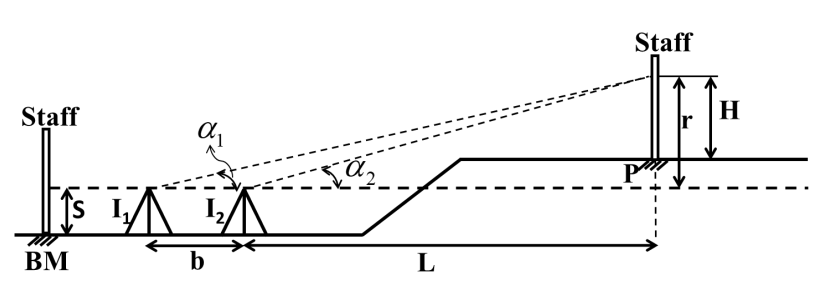
\includegraphics[width=0.7\columnwidth]{figs/fig9.png}
    \caption{\centering{Figure}}
    \label{figs:fig9}
\end{figure}
\begin{enumerate}
\item $L = \frac{b \tan{\alpha_1}}{\tan{\alpha_1} - \tan{\alpha_2}}$
\item $L = \frac{b \tan{\alpha_2}}{\tan{\alpha_1} - \tan{\alpha_2}}$
\item $L = \frac{b \tan{\alpha_1} \tan{\alpha_2}}{\tan{\alpha_1} - \tan{\alpha_2}}$
\item $L = \frac{b \tan{(\alpha_1 - \alpha_2)}}{\tan{\alpha_1} - \tan{\alpha_2}}$
\end{enumerate}
\hfill $\brak{\text{GATE GE 2025}}$
\bigskip
\item In a closed traversed with five sides, the closing error found from the fore bearing and back bearing of the last line is $+0.5\degree$. The correction to the fourth line will be
\begin{enumerate}
\begin{multicols}{4}
\item $-0\degree12'$
\item $0\degree18'$
\item $-0\degree24'$
\item $0\degree30'$
\end{multicols}
\end{enumerate}
\hfill $\brak{\text{GATE GE 2025}}$
\bigskip
\item Consider a pair of overlapping vertical aerial photographs taken from a flying height of $665$ m above a point A on the ground, with a camera having a focal length of $152.4$ mm. The height of the point A above the mean sea level is $535$ m. The parallax bar reading of the point A as measured from the photographs is $10.96$ mm. Assuming the air base to be $400$ m, the parallax bar constant is \rule{2cm}{0.5mm} mm.
\begin{enumerate}
\begin{multicols}{4}
\item $80.71$
\item $457.96$
\item $39.84$
\item $24.18$
\end{multicols}
\end{enumerate}
\hfill $\brak{\text{GATE GE 2025}}$
\bigskip
\item The statements below show the relationship of Whole Circle Bearing (WCB) with the Quadrantal Bearing (QB) for quadrant designations North-East (N-E), North West (N-W), South-East (S-E) and South-West (S-W). Which of the following statements is/are correct?
\begin{enumerate}
\item For the quadrant S-W, QB = WCB $-180\degree$
\item For the quadrant S-W, WCB = $180\degree -$ QB
\item For the quadrant N-W, WCB = $180\degree -$ QB
\item For the quadrant N-W, QB = $360\degree -$ WCB
\end{enumerate}
\hfill $\brak{\text{GATE GE 2025}}$
\bigskip
\item Consider an infinitely sized square grid pattern (as shown in the figure below) overlaid on a flat ground at an elevation of $120$ m above mean sea level. An image is taken by a camera from flying height of $450$ m above mean sea level. Assume that the flying height remains constant throughout the operation of the flight. The flying direction is along the line FL, as shown in the figure below. The camera is looking in the off-nadir in the flight direction resulting in a low oblique photograph. Which of the following statements for the resulting low oblique photograph is/are correct?
\begin{figure}[H]
    \centering
    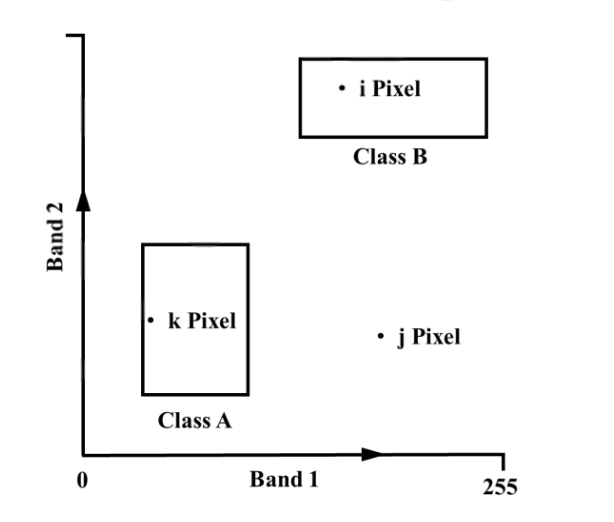
\includegraphics[width=0.2\columnwidth]{figs/fig11.png}
    \caption{\centering{Figure}}
    \label{figs:fig11}
\end{figure}
\begin{enumerate}
\item Scale of the photograph is not uniform along the flight direction
\item Parallel lines on the ground do not always appear parallel in the resulting photograph
\item Horizon is visible in the photograph
\item Cells A, B and C appear as squares in the resulting aerial photograph
\end{enumerate}
\hfill $\brak{\text{GATE GE 2025}}$
\bigskip
\item A point is specified along the Greenwich Meridian at $60\degree$ N latitude on an ellipsoid. The parameters of the ellipsoid are semi-major axis a=$6378137$ m and flattening factor $f = \frac{1}{298.257223563}$. The volume of the ellipsoid is given by $V_e = \frac{4}{3}\pi a^2 b$, where b is the semi-minor axis. The latitude of the point on the sphere whose volume is the same as the volume of the ellipsoid of reference is \rule{2cm}{0.5mm}\degree N $\brak{rounded\ off\ to\ 2\ decimal\ places}$.\\.
\hfill $\brak{\text{GATE GE 2025}}$
\bigskip
\item In a map based on the UTM projection, the grid distance is in error with respect to the geodetic distance by about one in four thousand. If the map distance is $3$ cm and the map scale is $1$:$25,000$, then the geodetic distance is \rule{2cm}{0.5mm} m $\brak{rounded\ off\ to\ 2\ decimal\ places}$.\\.
\hfill $\brak{\text{GATE GE 2025}}$
\bigskip
\item A level with the height of the instrument being $2.550$ m has been placed at a station having a Reduced Level (RL) of $130.565$ m. The instrument reads $3.665$ m on a levelling staff held inverted at the bottom of a bridge deck. The RL of the bottom of the bridge deck is \rule{2cm}{0.5mm} m $\brak{rounded\ off\ to\ 3\ decimal\ places}$.\\.
\hfill $\brak{\text{GATE GE 2025}}$
\bigskip
\item In levelling between two points P and Q on opposite banks of a river, the level was set up near P, and the staff reading on P and Q were $2.165$ m and $3.810$ m, respectively. The level was then moved and set up near Q and the respective staff readings on P and Q were $0.910$ m and $2.355$ m. The true difference of level between P and Q is \rule{2cm}{0.5mm} m $\brak{rounded\ off\ to\ 3\ decimal\ places}$.\\.
\hfill $\brak{\text{GATE GE 2025}}$
\bigskip
\item A $23$ cm square format camera with a focal length of $152.4$ mm is used for taking vertical aerial photographs with $60$\% end-lap. These photographs are viewed under a stereoscope with a base-height ratio of $0.15$. The vertical exaggeration while stereoviewing these photographs is \rule{2cm}{0.5mm} $\brak{Answer\ in\ integer}$.\\.
\hfill $\brak{\text{GATE GE 2025}}$
\bigskip
\end{enumerate}
\textbf{PART B2: FOR Image Processing and Analysis CANDIDATES ONLY}\\
\\
\textbf{Q.$66$ $-$ Q.$73$ Carry ONE mark Each}\\
\begin{enumerate}
\setcounter{enumi}{65}
\item Which one of the following image processing methods employs standard deviation?
\begin{enumerate}
\begin{multicols}{2}
\item Band ratio
\item Parallelepiped classification
\item Correction of skew distortion in raw satellite image
\item Nearest neighbor classification
\end{multicols}
\end{enumerate}
\hfill $\brak{\text{GATE GE 2025}}$
\bigskip
\item Which one of the following is NOT used to assess the quality of remote sensing image?
\begin{enumerate}
\begin{multicols}{2}
\item Univariate statistics of image
\item Histogram
\item Multivariate statistics of image
\item Swath of the image
\end{multicols}
\end{enumerate}
\hfill $\brak{\text{GATE GE 2025}}$
\bigskip
\item Which one of the following techniques is NOT used to atmospherically correct the satellite image?
\begin{enumerate}
\item Image normalization using histogram adjustment
\item Radiative transfer model
\item Image to image registration
\item Image normalization using regression
\end{enumerate}
\hfill $\brak{\text{GATE GE 2025}}$
\bigskip
\item A remote sensing instrument measures only in Green, Red and Near-Infrared frequency bands. The remote sensing index/indices that CANNOT be derived using data of this instrument is/are \rule{2cm}{0.5mm}.
\begin{enumerate}
\item Normalized Difference Vegetation Index
\item Atmospherically Resistant Vegetation Index
\item Soil Adjusted Vegetation Index
\item Enhanced Vegetation Index
\end{enumerate}
\hfill $\brak{\text{GATE GE 2025}}$
\bigskip
\item Principal Component Analysis is performed on a $4$-band IRS satellite image. The eigen values ($E = [\lambda_{1,1}, \lambda_{2,2}, \lambda_{3,3}, \lambda_{4,4}]$) computed from the covariance matrix are $887.60$, $75.20$, $37.60$ and $6.73$, respectively. The percentage of total variance explained by the third principal component ($\lambda_{3,3}$) is \rule{2cm}{0.5mm} $\brak{rounded\ off\ to\ 2\ decimal\ places}$.\\.
\hfill $\brak{\text{GATE GE 2025}}$
\bigskip
\item Piecewise linear contrast stretch is performed on an $8$-bit image. The output ($BV_{out}$) would be zero for input value $BV_{in} \le 80$. The output ($BV_{out}$) would be $255$ for $BV_{in} > 120$. For the remaining input values, $BV_{out} = (2 \times BV_{in}) - 20$. If $BV_{in} = 120$, then $BV_{out}$ is \rule{2cm}{0.5mm} $\brak{Answer\ in\ integer}$.\\.
\hfill $\brak{\text{GATE GE 2025}}$
\bigskip
\item A CCD array element in a remote sensing sensor measures incoming radiation and its output voltage varies linearly between $0$ V to $5$ V. This voltage is converted to an $8$-bit digital image using an analogue to digital convertor (ADC). The ADC has a linear response without bias or noise. If the output image pixel has a digital number of $100$, the input voltage to the ADC would be \rule{2cm}{0.5mm} V $\brak{rounded\ off\ to\ 2\ decimal\ places}$.\\.\\
\hfill $\brak{\text{GATE GE 2025}}$
\bigskip
\item In supervised digital image classification, the number of combinations to be evaluated to select three best bands out of five bands is \rule{2cm}{0.5mm} $\brak{Answer\ in\ integer}$.\\.
\hfill $\brak{\text{GATE GE 2025}}$
\bigskip
\end{enumerate}
\textbf{Q.$74$ $-$ Q.$84$ Carry TWO marks each}\\
\begin{enumerate}
\setcounter{enumi}{73}
\item The figure below shows a one-dimensional function, $f$, and a filter $w$. Consider $f$ is padded with zeros on both sides. Which one among the following will be the final convolution output of $f$ with $w$ after the padding zeros are removed from the output?
\begin{figure}[H]
    \centering
    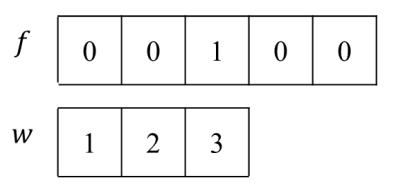
\includegraphics[width=0.4\columnwidth]{figs/fig12.png}
    \caption{\centering{Figure}}
    \label{figs:fig12}
\end{figure}
\begin{enumerate}
\item 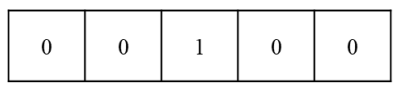
\includegraphics[width=0.4\columnwidth]{figs/fig15.png}
\item 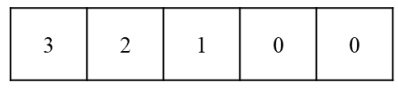
\includegraphics[width=0.4\columnwidth]{figs/fig16.png}
\item 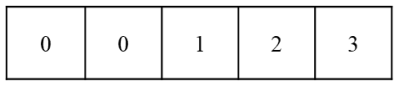
\includegraphics[width=0.4\columnwidth]{figs/fig17.png}
\item 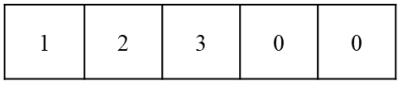
\includegraphics[width=0.4\columnwidth]{figs/fig18.png}
\end{enumerate}
\hfill $\brak{\text{GATE GE 2025}}$
\bigskip
\item Figure below shows the scatterplot of training pixels of water (w), sand (s), forest (f) and commercial (c) in bands 1 and 2. Pixel ‘A’ having digital number 4 and 6 in band 1 and band 2, respectively, is to be classified using k-nearest neighbor classifier having the value of k equal to 5. The assigned class for the pixel ‘A’ is \rule{2cm}{0.5mm}.
\begin{figure}[H]
    \centering
    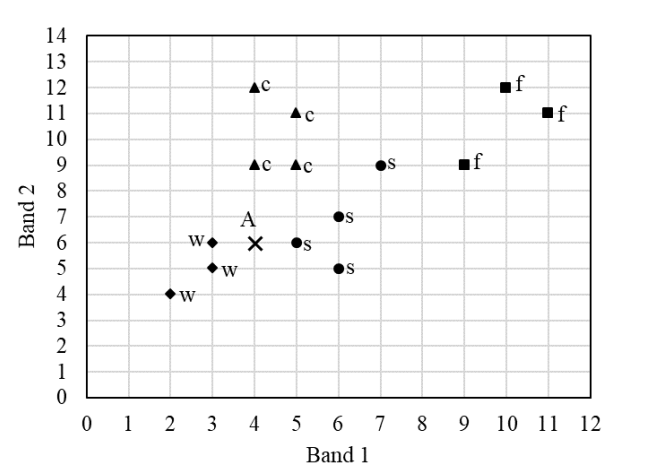
\includegraphics[width=0.6\columnwidth]{figs/fig13.png}
    \caption{\centering{Figure}}
    \label{figs:fig13}
\end{figure}
\begin{enumerate}
\begin{multicols}{4}
\item forest
\item sand
\item water
\item commercial
\end{multicols}
\end{enumerate}
\hfill $\brak{\text{GATE GE 2025}}$
\bigskip
\item A remote sensing image is acquired from an IRS series satellite. Initially a two dimensional filter with transfer function $H(u, v) = \exp \left(-\frac{D^2(u,v)}{2D_0^2}\right)$ is applied to reduce scan line effects. Here $D(u, v)$ is the distance from center of the frequency rectangle, and $D_0$ is the cutoff frequency. Which one of the following will be the transfer function for the corresponding filter to detect the edges in the image?
\begin{enumerate}
\item $1 - \exp \left(-\frac{D^2(u, v)}{2D_0^2}\right)$
\item $\exp \left(-\frac{D^2(u, v)}{2D_0^2}\right)$
\item $1 + \exp \left(-\frac{D^2(u, v)}{2D_0^2}\right)$
\item $1 - \exp \left(\frac{D^2(u, v)}{2D_0^2}\right)$
\end{enumerate}
\hfill $\brak{\text{GATE GE 2025}}$
\bigskip
\item Consider an imaging system with $N \times N$ pixels that produces a noiseless, distortion-free digital image. It is used to digitize checkerboard patterns where all squares of the pattern are in the field of view. Using this imaging system, if a checkerboard pattern with $M \times M$ squares is digitized, each square will be $N/M \times N/M$ pixel in size. What is the size of the checkerboard square in the generated digital image for which spatial aliasing is observed (measured in pixels of the imaging system)?
\begin{enumerate}
\begin{multicols}{4}
\item $1$
\item $2$
\item $0.9$
\item $2.5$
\end{multicols}
\end{enumerate}
\hfill $\brak{\text{GATE GE 2025}}$
\bigskip
\item For the correlation matrix of a 4-band satellite image as shown below, which of the following statements is/are correct?
\begin{table}[H]
\centering
\begin{tabular}{|c|c|c|c|c|}
\hline
\textbf{} & \textbf{Band 1} & \textbf{Band 2} & \textbf{Band 3} & \textbf{Band 4} \\ \hline
\textbf{Band 1} & 1.00 & 0.91 & 0.32 & 0.88 \\ \hline
\textbf{Band 2} & 0.91 & 1.00 & 0.25 & 0.98 \\ \hline
\textbf{Band 3} & 0.32 & 0.25 & 1.00 & 0.22 \\ \hline
\textbf{Band 4} & 0.88 & 0.98 & 0.22 & 1.00 \\ \hline
\end{tabular}
\end{table}
\begin{enumerate}
\item Band 3 provides some unique information not found in other bands
\item There is high redundancy in band 2 and 4
\item The standard deviation of all the bands is equal
\item Image cannot be classified using bands 1 and 3 only
\end{enumerate}
\hfill $\brak{\text{GATE GE 2025}}$
\bigskip
\item The histogram of a red band in a 3-bit satellite image is shown below. Which of the following statements is/are correct?
\begin{figure}[H]
    \centering
    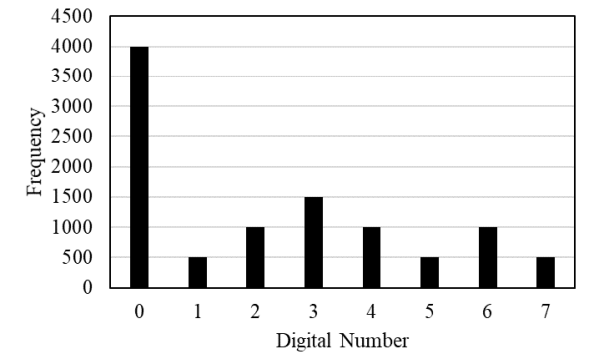
\includegraphics[width=0.6\columnwidth]{figs/fig14.png}
    \caption{\centering{Figure}}
    \label{figs:fig14}
\end{figure}
\begin{enumerate}
\item There are more darker pixels in the image
\item There are more brighter pixels in the image
\item The mean digital number of the image is 1250
\item It may be predicted that approximately 40\% of area in the image is covered by material with low spectral albedo in red band
\end{enumerate}
\hfill $\brak{\text{GATE GE 2025}}$
\bigskip
\item Which of the following statements is/are correct regarding across-track scanning sensor of an airborne optical imaging system?
\begin{enumerate}
\item The relief displacement will be along the direction of the flight line
\item There is no relief displacement along the direction of the flight line
\item The greater is the distance of the ground object from nadir, the lesser is the image scale compression
\item Linear features have sigmoidal distortion
\end{enumerate}
\hfill $\brak{\text{GATE GE 2025}}$
\bigskip
\item In case of normalized difference vegetation index (NDVI), which of the following statements is/are correct?
\begin{enumerate}
\item It is functionally equivalent to a simple ratio of red to near infra-red reflectance
\item It reduces many forms of multiplicative noise
\item It reduces additive noise
\item It is sensitive to canopy background variations
\end{enumerate}
\hfill $\brak{\text{GATE GE 2025}}$
\bigskip
\item The hue, intensity and saturation values for a pixel are $H = 0.5$ rad, $S = 0.5$ and $I = 0.3$, respectively. If the pixel is converted to RGB color model, then the value of the green pixel would be \rule{2cm}{0.5mm} $\brak{rounded\ off\ to\ 2\ decimal\ places}$.
\\.
\hfill $\brak{\text{GATE GE 2025}}$
\bigskip
\item The brightness values of four pixels in the input image are shown in the table below. The image is rectified using nearest neighbor intensity interpolation, and the pixel at location (5, 4) in the output image is to be filled with the value from coordinate (5.3, 3.7) in the input image. The brightness value of the pixel at location (5, 4) in the rectified output image is \rule{2cm}{0.5mm} $\brak{Answer\ in\ integer}$.
\begin{table}[H]
\centering
\begin{tabular}{|c|c|}
\hline
\textbf{Location} & \textbf{Brightness Value} \\ \hline
(5, 3) & 100 \\ \hline
(6, 3) & 120 \\ \hline
(5, 4) & 110 \\ \hline
(6, 4) & 130 \\ \hline
\end{tabular}
\end{table}
\hfill $\brak{\text{GATE GE 2025}}$
\bigskip
\item The error matrix resulting from randomly selected test pixels for a classified image is given below. The Producer’s accuracy of class 1 is \rule{2cm}{0.5mm} \% $\brak{rounded\ off\ to\ 1\ decimal\ place}$.
\begin{table}[H]
\centering
\begin{tabular}{|c|c|ccc|c|}
\hline
\multicolumn{2}{|c|}{\multirow{2}{*}{}} & \multicolumn{3}{c|}{\textbf{Reference Data}} & \multirow{2}{*}{\textbf{Total}} \\ \cline{3-5}
\multicolumn{2}{|c|}{} & \textbf{C1} & \textbf{C2} & \textbf{C3} & \\ \hline
\multirow{3}{*}{\textbf{\begin{tabular}[c]{@{}c@{}}Classified\\ Data\end{tabular}}} & \textbf{C1} & 100 & 10 & 5 & 115 \\
& \textbf{C2} & 8 & 120 & 12 & 140 \\
& \textbf{C3} & 2 & 5 & 80 & 87 \\ \hline
\multicolumn{2}{|c|}{\textbf{Total}} & 110 & 135 & 97 & 342 \\ \hline
\end{tabular}
\end{table}
\hfill $\brak{\text{GATE GE 2025}}$
\bigskip
\end{enumerate}


\end{document}